\subsection{Salvataggio test}

\begin{figure}[H]
    \centering
    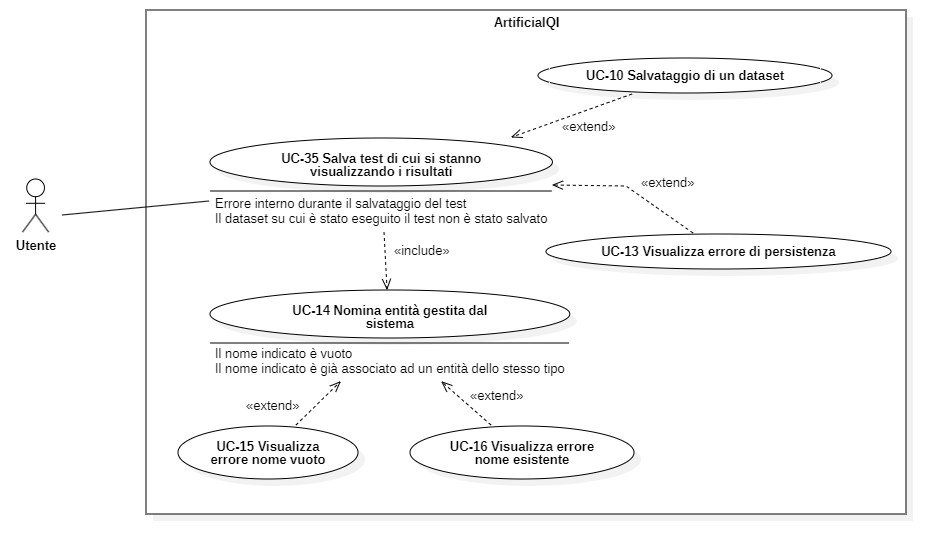
\includegraphics[scale=0.2]{Sezioni/UseCase/Immagini/SalvataggioTest.png}
    \caption{Salvataggio test.}
\end{figure}

\begin{usecase}{UC-38}{Salva test di cui si stanno visualizzando i risultati}
    \label{uc:UC-38}
    
    \req{RUF-1} 

    \pre{
        \item L'utente sta visualizzando i risultati del test da salvare
        \item Il test è sono ancora stato salvato nel sistema
    }

    \post{
        \item I risultati del test vengono salvati nel sistema
    }
    
    \actor{Utente}

    \subactors{}

    \trigger{L'utente vuole salvare i risultati del test}

    \inc{\hyperref[uc:UC-17]{UC-17}}

    \base{}

    \scenario{
        \item L'utente richiede di salvare il test
        \item Il sistema ottiene il nome per il nuovo test seguendo \hyperref[uc:UC-17]{UC-17}
        \item Il sistema verifica che il dataset su cui è stato eseguito il test è già stato salvato
        \item Il sistema salva il test 
        \item Il sistema notifica l'utente del corretto salvataggio
    }

    \subscenario{
        \item[3.1] Il dataset su cui è stato eseguito il test non è stato salvato:
        \begin{itemize}
            \item \hyperref[uc:UC-12]{UC-12}
        \end{itemize}
        \item[4.1] Il sistema verifica un errore interno durante il salvataggio del test:
        \begin{itemize}
            \item \hyperref[uc:UC-16]{UC-16}
        \end{itemize}
    }
\end{usecase}

